%%%%%%%%%%%%%%%%%%%%%%%%%%%%%%%%%%%%%%%%%
% The Legrand Orange Book
% LaTeX Template
% Version 2.1.1 (14/2/16)
%
% This template has been downloaded from:
% http://www.LaTeXTemplates.com
%
% Original author:
% Mathias Legrand (legrand.mathias@gmail.com) with modifications by:
% Vel (vel@latextemplates.com)
%
% License:
% CC BY-NC-SA 3.0 (http://creativecommons.org/licenses/by-nc-sa/3.0/)
%
% Compiling this template:
% This template uses biber for its bibliography and makeindex for its index.
% When you first open the template, compile it from the command line with the 
% commands below to make sure your LaTeX distribution is configured correctly:
%
% 1) pdflatex main
% 2) makeindex main.idx -s StyleInd.ist
% 3) biber main
% 4) pdflatex main x 2
%
% After this, when you wish to update the bibliography/index use the appropriate
% command above and make sure to compile with pdflatex several times 
% afterwards to propagate your changes to the document.
%
% This template also uses a number of packages which may need to be
% updated to the newest versions for the template to compile. It is strongly
% recommended you update your LaTeX distribution if you have any
% compilation errors.
%
% Important note:
% Chapter heading images should have a 2:1 width:height ratio,
% e.g. 920px width and 460px height.
%
%%%%%%%%%%%%%%%%%%%%%%%%%%%%%%%%%%%%%%%%%

%----------------------------------------------------------------------------------------
%	PACKAGES AND OTHER DOCUMENT CONFIGURATIONS
%----------------------------------------------------------------------------------------

\documentclass[11pt,fleqn]{book} % Default font size and left-justified equations

\usepackage{ifthen} 
\newboolean{VersionProf}
\setboolean{VersionProf}{false}

\usepackage{wasysym}
\usepackage{esint} % various fancy integral symbols
\usepackage{tikz}
\usepackage{tikz-3dplot}
\usepackage{pgfplots}
\pgfplotsset{compat=1.17}
\usetikzlibrary{patterns}
\usepackage{tkz-euclide} 
\usepackage{mathtools}
\usepackage{xurl}
\usepackage[version=4,arrows=pgf-filled,
textfontname=sffamily,
mathfontname=mathsf]{mhchem}
\usepackage{gensymb}
\usepackage{tabularray}
\usepackage{csquotes}

\usepackage[french]{babel}
\usepackage{dingbat}

\usepackage{environ}
\usepackage{wrapfig}

\NewEnviron{solution}{%
    \ifthenelse{\boolean{VersionProf}}{\begin{solutionA}
        \BODY%*
        \end{solutionA}
    }{%
        \relax%
    }%
}%

\usetikzlibrary {arrows.meta} 

\newcommand{\degC}{{\degree}C}
\newcommand{\dd}{\mathrm{d}}
\newcommand{\div}{\mathrm{div}}
\newcommand{\rot}{\vv{\mathrm{div}}}
\newcommand{\grad}{\vv{\mathrm{grad}}}

\tikzset{
    support/.style={
        pattern=north east lines,
        draw=none,
        minimum width=0.3,
        minimum height=0.6
    }
    ,>=latex
}

\usepackage[d]{esvect}

%SPECIFIC TO THIS CHAPTER
\usepackage{physics}
\usepackage{ifthen}
\usepackage[outline]{contour} % glow around text
\usetikzlibrary{calc} % for pic
\usetikzlibrary{angles,quotes} % for pic
\usetikzlibrary{patterns}
\tikzset{>=latex} % for LaTeX arrow head
\contourlength{1.2pt}

\colorlet{myred}{red!65!black}
\definecolor{myred}{RGB}{127,0,255}
\tikzstyle{ground}=[preaction={fill,top color=black!10,bottom color=black!5,shading angle=20},
                    fill,pattern=north east lines,draw=none,minimum width=0.3,minimum height=0.6]
\tikzstyle{mass}=[line width=0.6,myred,fill=myred!40,rounded corners=1,
                  top color=myred!40,bottom color=myred!20,shading angle=20]
\tikzstyle{rope}=[myred!30,line width=1.2,line cap=round] %very thick

% FORCES SWITCH
\tikzstyle{force}=[->,myred,ultra thick,line cap=round]
\tikzstyle{Fproj}=[force,myred!60]
\newboolean{showforces}
\setboolean{showforces}{true}
%----------------------------------------------------------------------------------------

\input{structure} % Insert the commands.tex file which contains the majority of the structure behind the template

\begin{document}

%----------------------------------------------------------------------------------------
%	TABLE OF CONTENTS
%----------------------------------------------------------------------------------------

%\usechapterimagefalse % If you don't want to include a chapter image, use this to toggle images off - it can be enabled later with \usechapterimagetrue

\chapterimage{filmB.jpg} % Table of contents heading image

%\pagestyle{empty} % No headers

%\tableofcontents % Print the table of contents itself

%\cleardoublepage % Forces the first chapter to start on an odd page so it's on the right

%\pagestyle{fancy} % Print headers again



%\part{\'{E}lectromagnétisme}

\setcounter{chapter}{13}

\chapter{Cinétique électrochimique}

Nous avons vu, à travers les diagrammes potentiel-pH notamment, tous les aspects thermodynamiques des réactions électrochimiques. Cependant, certains processus ne s'expliquent pas par une description purement thermodynamique : certaines réactions qui devraient être thermodynamiquement favorisées ne se font pas, et on constate également que la corrosion des métaux est généralement non uniforme, mais que les métaux sont souvent plus attaqués à des endroits spécifiques.

Pour comprendre ces phénomènes, nous allons dans un premier temps montrer que la cinétique des réactions électrochimiques est reliée au courant électrique qui arrive ou part de la zone dans laquelle la réaction se produit (typiquement, une électrode ou une région soumise à la corrosion). Nous expliquerons ensuite de manière phénoménologique les différents facteurs influençant la vitesse de la réaction chimique.

\section{Mesure expérimentale de la vitesse de réaction}

\subsection{Vitesse de réaction}

On considère une électrode, à laquelle arrive un courant $i$. Par convention, $i$ est compté positivement lorsqu'il arrive à l'électrode. On suppose que la réaction électrochimique se produisant au niveau de l'électrode fait intervenir un couple rédox tel que :
\begin{equation}
	\alpha Ox + n e^- = \beta Red
\end{equation}

\begin{capex}
	Montrer que l'intensité arrivant à l'électrode est proportionnelle à la vitesse de la réaction. On étudiera séparément le cas d'une oxydation et d'une réduction.
\end{capex}

En pratique, on pourra donc directement mesurer la vitesse d'une réaction électrochimique à l'aide d'un ampèremètre, ce qui rend les études cinétiques nettement plus simples sur des réactions électrochimiques se produisant à une électrode que sur la plupart des réactions en solution aqueuse.

\subsection{Montage à trois électrodes}

Pour mesurer le courant $i$, on utilise un montage particulier appelé le montage à trois électrodes, qui va nous permettre de réaliser une mesure en contrôlant les conditions dans lesquelles se fait la réaction, et en particulier de tracer le courant $i$ en dfonction du potentiel de l'électrode. On utilise les électrodes suivantes :
\begin{itemize}
	\item Une électrode de travail : c'est sur cette électrode que se produit la réaction chimique qui nous intéresse ;
	\item Une électrode de référence, dont le potentiel est connu précisément (on pourra ainsi mesurer la différence de potential entre l'électrode de référence et l'électrode de travail) ;
	\item Une contre-électrode servant à fermer le circuit électrique (sinon, les électrons ne peuvent pas circuler).
\end{itemize}

\begin{figure}[htbp]
	\centering 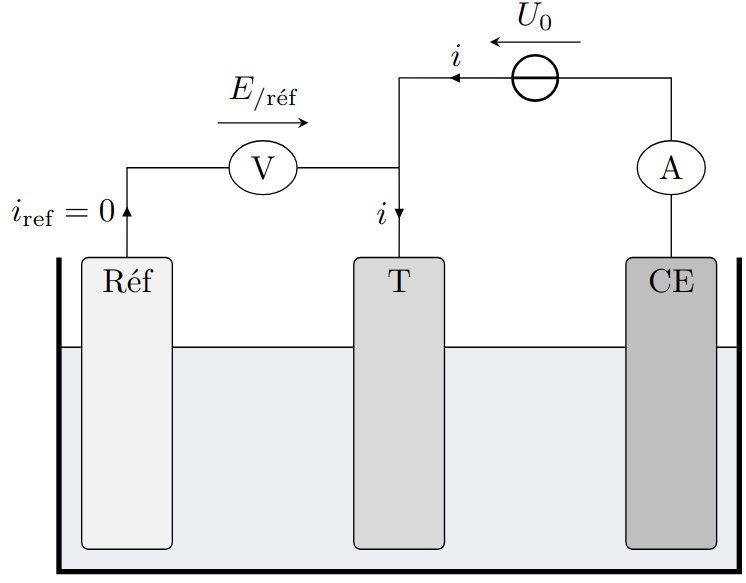
\includegraphics[width=0.75\linewidth]{montage_3_electrodes.png}
	\caption{Montage à trois électrodes. Source : ploy de cours de Etienne Thibierge.}
\end{figure}

Nous allons nous intéresser plus précisément à ces trois électrodes :

\paragraph{Electrode de travail}

L'électrode de travail peut être utilisée comme cathode ou comme anode, selon la nature de la réaction électrochimique qui s'y produit (oxydation ou réduction). La nature de l'électrode peut dépendre de la réaction qui s'y produit :
\begin{itemize}
	\item Dans le cas d'une réaction entre un métal et un cation métallique, on choisit souvent une électrode constituée du métal en question, on parle alors d'une électrode de première espèce. De la matière peut alors être ajoutée ou retirée à l'électrode lorsque la réaction se produit. C'est le cas, par exemple, d'une électrode en fer dans une réaction qui fait intervenir le couple $\ce{Fe^{2+}(aq) / Fe(s)}$.
	\item Dans d'autres cas, l'électrode est constituée d'un pétal interte comme le platine. Les composés qui réagissent sont en solution ou gazeux et l'électrode agitu uniquement comme un support de la réaction, par lequel les électrons peuvent être fournis ou extraits de la solution aqueuse. On parle alors d'une électrode de 3e espèce. C'est le cas, par exemple, d'une électrode de platine sur laquelle l'eau est réduite en dihydrogène (couple $\ce{H^+(aq) / H2(g))}$).
\end{itemize}

\paragraph{Electrode de référence} Afin de connaître le potentiel de l'électrode de travail, il est nécessaire de mesurer la tension entre l'électrode de travail et une électrode de référence dont le potentiel est connu. Par convention le potentiel standard du couple $\ce{H^+(aq) / H2(g))}$ est fixé à 0\,V, et l'électrode standard à hydrogène est une électrode dont le potentiel devrait toujours être égal à 0\,V.  Cette électrode étant en pratique très difficile à réaliser, on utilise plutôt d'autres électrodes de référence comme l'électrode au calomel saturé. Le concept de ces électrodes est simple : le potentiel de l'électrode est donné par la loi de Nernst et dépend de la concentration en ions. Néanmoins, cette concentration peut être fixée en s'assurant que l'on a dans l'électrode une soluton saturée, ce qui fixe la concentration des ions en question.

\begin{figure}[htbp]
	\centering 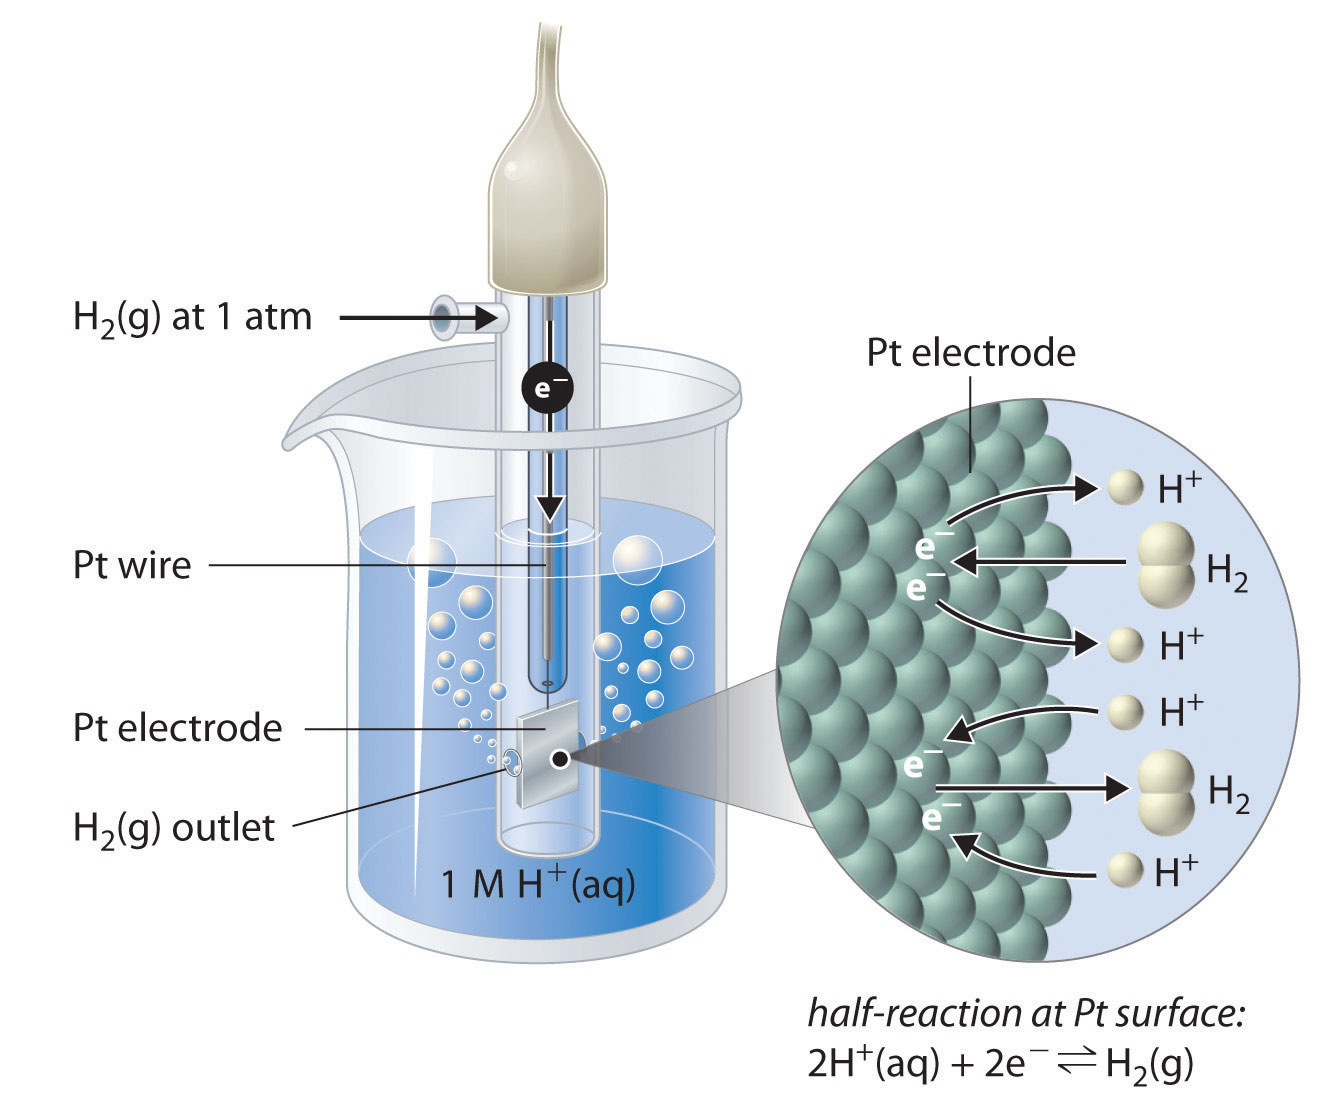
\includegraphics[width=0.65\linewidth]{electrode_hydrogene.jpg} 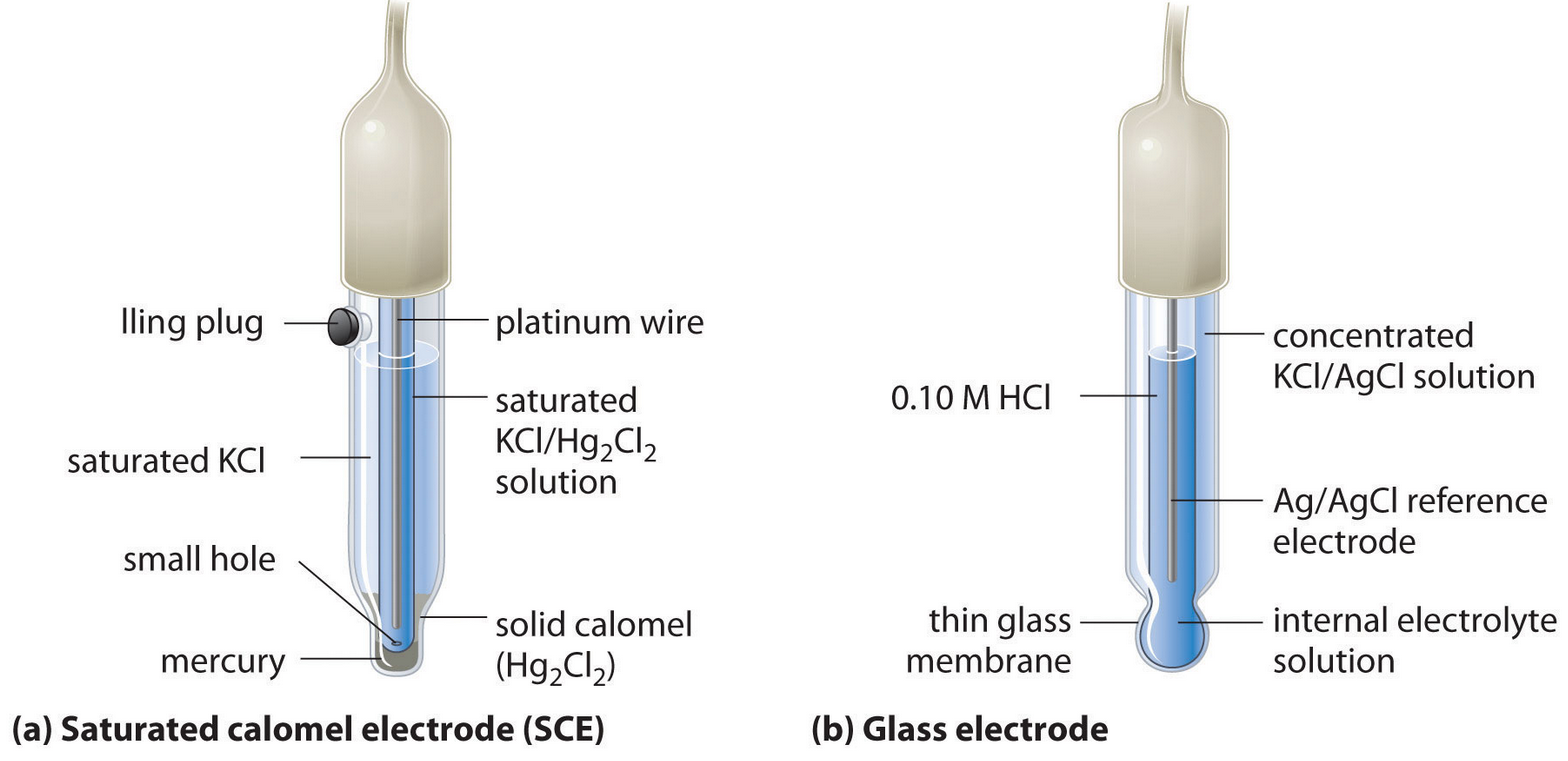
\includegraphics[width=\linewidth]{electrodes_de_reference.png}
	\caption{En haut : électrode standard à hydrogène (électrode théorique dont le potentiel serait égal à 0\,V). En bas : deux électrodes de référence usuelles : l'électrode au calomel saturé et l'électrode de verre. Source : Saylor Academy.}
\end{figure}

\paragraph{Contre-électrode} La contre-électrode sert à fermer le circuit électrique. En effet, puisque l'on place un voltmètre entre l'électrode de référence et l'électrode de travail, aucun courant ne peut circuler entre ces électrodes. En général, on choisit une électrode inerte. On prend une électrode de grande surface pour que la vitesse de la réaction qui se produit à sa surface ne soit pas limitée. 

Le montage à trois électrodes, en règle générale, peut directement être réalisé à l'aide d'un potentiostat conçu directement à cet effet. On peut choisir le potentiel de l'électrode de travai : celui-ci est réglé automatiquement par le potentiostat via un asservissement utilisant la mesure du voltmètre. L'appareil fournit alors une mesure du courant.

\subsection{Courbes courant-potentiel}

\begin{definition}
	On appelle courbe courant-potentiel $i(E)$ la courbe indiquant l'intensité électrique $i$ arrivant à l'électrode de travail en fonction du potentiel de l'électrode. 
\end{definition}

On constate expérimentalement que cette courbe dépend :
\begin{itemize}
	\item Du couple rédox qui réagit au niveau de l'électrode ;
	\item De la surface immergée de l'électrode ;
	\item De la nature de l'électrode ;
	\item De la nature du solvant.
\end{itemize}

On remarque également la propriété suivante :
\begin{proposition}
	La courbe $i(E)$ est toujours positive (oxydation) lorsque le potentiel est supérieur au potentiel de Nernst du couple, et négative (réduction) sinon.
\end{proposition} 

Cette propriété s'explique par la formule de Nernst : lorsqu'un impose un potentiel $E'$, le système cherche à évoluer vers un nouvel équilibre tel que $E = E'$, or :
\begin{equation}
	E = E^\circ(Ox/Red) + \frac{0.06}{n} \log \left( \frac{a(Ox)^\alpha}{a(Red)^\beta} \right)
\end{equation}
Si le potentiel $E'$ est supérieur au potentiel d'équilibre, le réducteur va donc être converti en oxydant ce qui va augmenter le second terme de l'équation : on aura donc une oxydation. Le courant $i$ sera ainsi positif.

On constate que la courbe $i(E)$ présente différentes allures selon les configurations.

\subsection{Système rapide}

Dans le cas d'un système rapide, l'application d'un potentiel différent du potentiel d'équilibre conduit immédiatement à l'apparition d'une réaction. 

\begin{definition}
	On définit le surpotentiel $\eta$ (parfois également appelé surtension) comme l'écart entre le potentiel à appliquer et le potentiel de Nernst afin d'avoir un courant $i$. Il est toujours pris positif :
	\begin{equation}
		\eta(i) = |E(i) - E_{\rm Nernst}|
	\end{equation}
	
\end{definition}

On constate que le courant (en valeur absolue) augmente avec le surpotentiel : plus on se place loin de l'équilibre et plus la vitesse de la réaction chimique est rapide. 

\begin{figure}[htbp]
	\centering 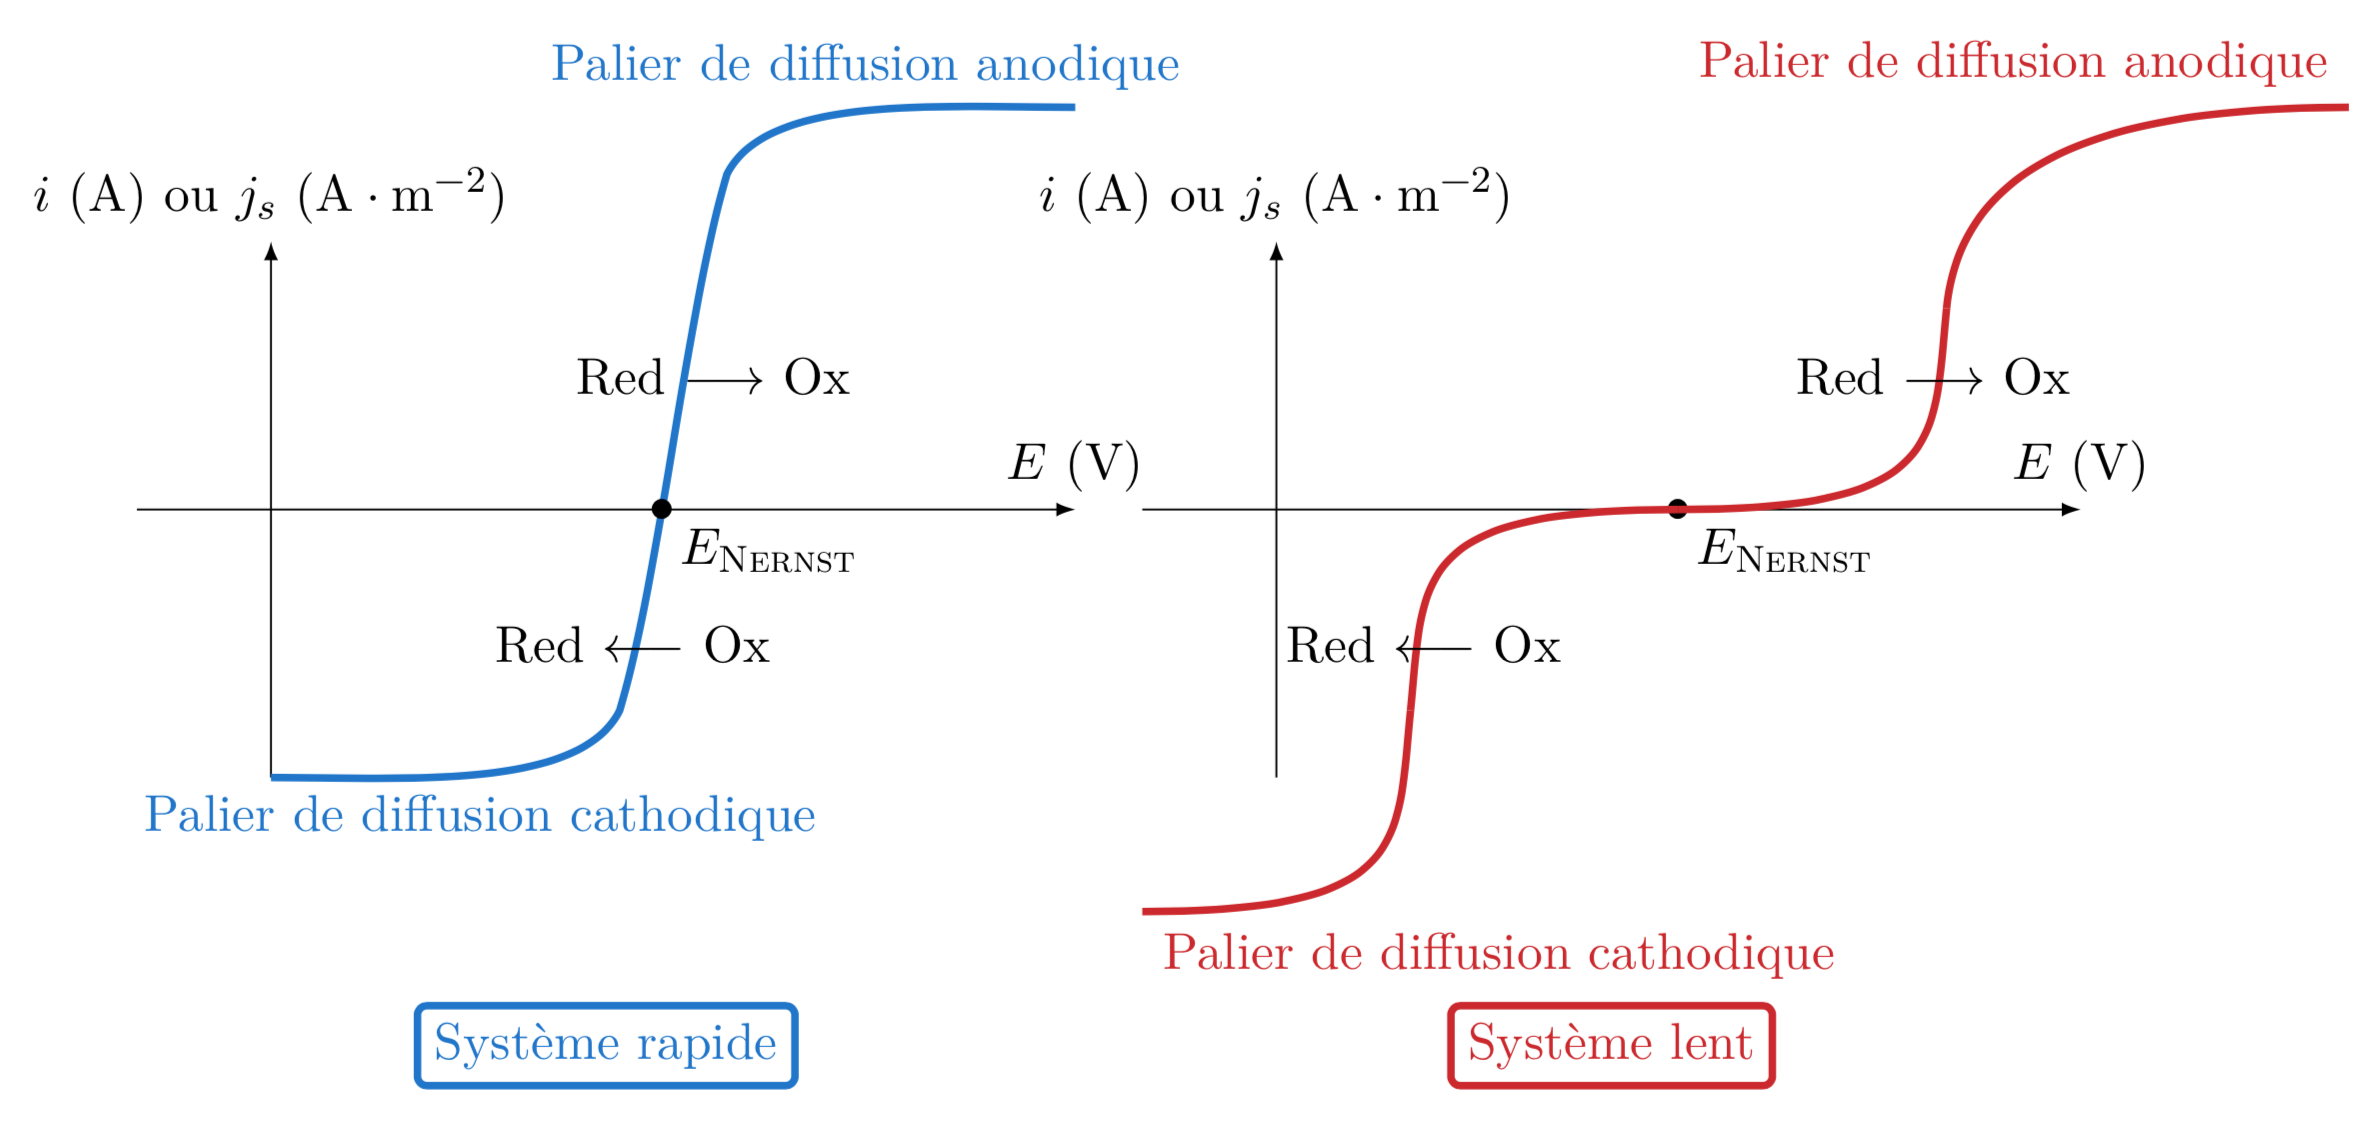
\includegraphics[width=\linewidth]{systeme_rapide_lent.png}
	\caption{Courbes courant-potentiel d'un système rapide (à gauche) et lent (à droite). On considère dans les deux cas un couple rédox entre deux ions, par exemple $\ce{Fe^{3+} / Fe^{2+}}$. Source : pt.physique.free.fr}
\end{figure}

\subsection{Système lent}

Dans le cas de certains systèmes ou de certaines électrodes, on observe que la courbe $i(E)$ est nulle ou quasi nulle au voisinage du potentiel de Nernst. On parle alors d'un système lent :
\begin{definition}
	Un système est dit lent lorsqu'il faut appliquer une surtension non nulle afin de réaliser une réaction électrochimique. 
	
	On appelle alors surpotentiel à vide (ou à courant nul) le surpotentiel à imposer pour que l’intensité devienne non nulle.
	On distingue le surpotentiel anodique (pour une oxydation ; $E>E_{\rm Nernst}$ et $i>0$) et le surpotentiel cathodique (pour une réduction ; $E<E_{\rm Nernst}$ et $i<0$).
\end{definition}

En pratique, ce phénomène traduit la cinétique du transfert de charge : il est nécessaire d'appliquer une différence de potentiel non nulle entre l'électrode et la solution aqueuse pour que les électrons puissent se déplacer de l'un à l'autre. Ceci implique que la réaction ne peut pas se produire tant que le surpotentiel ne dépasse pas une valeur critique non nulle. 

\begin{remark}
	La valeur du surpotentiel à vide dépend de l'électrode utilisée, et certaines électrodes permettent de réduire fortement ce surpotentiel. On en voit un exemple dans le cas de la réduction de l'eau en dihydrogène.
\end{remark}

\begin{figure}[htbp]
	\centering 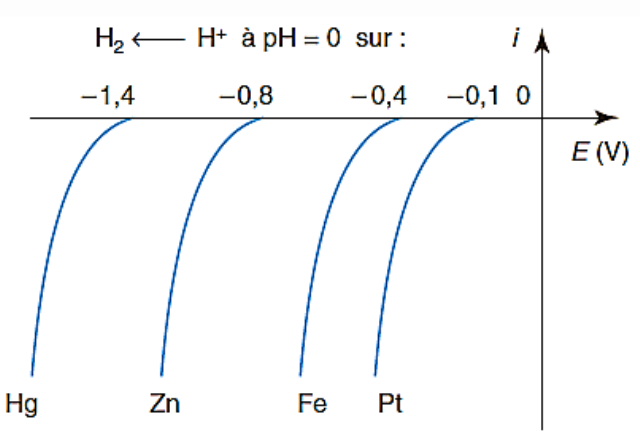
\includegraphics[width=0.55\linewidth]{reduction_eau.png}
	\caption{Courbes courant-potentiel correspondant à la réduction de l'eau sur différentes électrodes. Source : poly de cours de Virginie Sablonière.}
\end{figure}


\subsection{Palier de diffusion}

On observe que, dans le cas où l'un ou plusieurs des réactifs sont une espèce en solution, à partir d'un certain surpotentiel appliqué, la vitesse de la réaction n'augmente plus : on parle alors de palier de diffusion.

Ce palier de diffusion s'explique par le phénomène de diffusion : les ions consommés au niveau de l'électrode doivent se déplacer depuis la solution vers l'électrode par diffusion à une vitesse suffisante, avant de venir s'adsorber sur l'électrode où la réaction se produit. La quantité d'ions pouvant arriver sur l'électrode par unité de temps est généralement proportionnelle à :
\begin{itemize}
	\item La surface immergée $S$ de l'électrode.
	\item La concentration en ions réactifs dans la solution $c$.
	\item La charge de l'ion réactif.
\end{itemize}

\begin{figure}[htbp]
	\centering 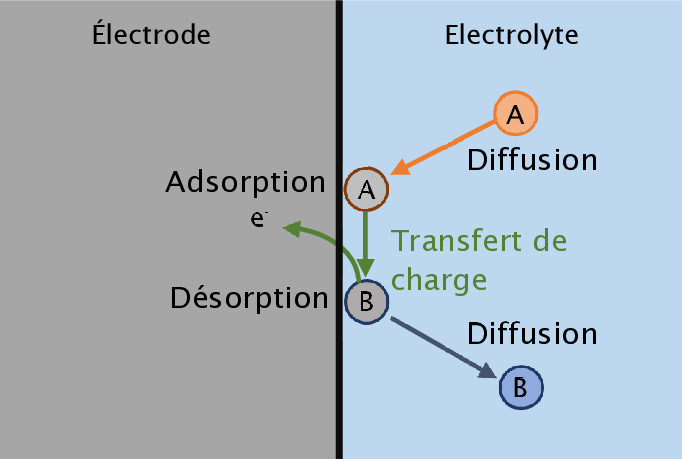
\includegraphics[width=0.55\linewidth]{palier_diffusion.png}
	\caption{Les processus microscopiques intervenant au voisinage de l'électrode dans le cas d'une réaction d'oxydation d'un composé $A$ en un composé $B$ . Source : thèse de Mathieu Robineau.}
\end{figure}

\begin{capex}
	Tracer l'allure de la courbe $i(E)$ pour le couple $\ce{Cu^{2+}(aq) / Cu(s)}$, suru une électrode de cuivre, sachant que le couple est rapide. Quelle est l'allure de la courbe si on double la concentration en ions cuivre (II) dans la solution ? Si on double la surface immergée de l'électrode ?
\end{capex}

\subsection{Courbe courant-potentiel en prèsence de plusieurs espèces}

Les réactions chimiques ne sont a priori pas en compétition les unes avec les autres, on peut plutôt considérer qu'elles sont relativement indépendantes. On en déduit la propriété suivante :
\begin{proposition}
	Lorsque plusieurs couples peuvent réagir à une même électrode, les intensités de chaque réaction électrochimique s’ajoutent.
\end{proposition}


On constate que s'il n'y a pas de palier de diffusion, la formation des oxydants les plus puissants et des réducteurs les plus puissants est inhibée. En particulier, les intensités liées à l'oxydation et la réduction de l'eau ne présentent pas de palier de diffusion, et forment ce que l'on appelle le "mur du solvant" :
\begin{definition}
	Le mur du solvant correspond aux deux vagues d'oxydation et de réduction de l'eau. Le domaine compris entre ces deux vagues est appelé domaine d'inertie électrochimique ; il n'est pas possible de porter la solution à un potentiel en dehors de ce domaine.
\end{definition}

\section{Application à la corrosion humide}

\subsection{Notion de potentiel mixte}

\begin{capex}
	On considère un clou en fer solide situé dans une solution acide. Tracer l'allure des courbes intensité-potentiel au niveau du clou, ainsi que l'intensité totale.
\end{capex}

Dans un système naturel, le montage à trois électrodes n'existe pas, et un objet métallique doit garder sa neutralité électrique. Le courant qui s'échappe de l'objet doit donc nécessairement être nul, ce qui impose la valeur du potentiel pour que $i=0$ :
\begin{definition}
	On appelle potentiel mixte $E_{\rm mix}$ le potentiel tel que le courant total arrivant au niveau d'un objet métallique ou d'une électrode est nul ($i=0$).
\end{definition}

\begin{capex}
	A partir de l'allure des courbes courant-potentiel, interpréter ce qui se passe dans la solution. Quels facteurs vont favoriser la corrosion du métal ?
\end{capex}

\subsection{Blocage cinétique}

Parfois, une réaction qui devrait se produire thermodynamiquement ne se produit pas pour des raisons cinétiques, c'est ce que l'on appelle le blocage cinétique. On peut prendre l'exemple de la corrosion du zinc en milieu acide. Les courbes $i(E)$ ci-dessous indiquent que si le zlinc est pur, le surpotentiel nécessaire pour oxyder le zinc est tel que la réaction avec l'eau ne peut plus se produire, et le zinc reste alors sous état solide. Si le zinc est impur en revanche, le surpotentiel à vide est plus faible et la réaction de corrosion peut se produire.

\begin{remark}
	Dans ce cas, on ne peut pas définir clairement de potentiel mixte puisqu'il existe une plage de potentiels qui vérifient la conditon $i=0$, mais on peut conclure qu'aucune réaction ne se produit.
\end{remark}


\begin{figure}[htbp]
	\centering 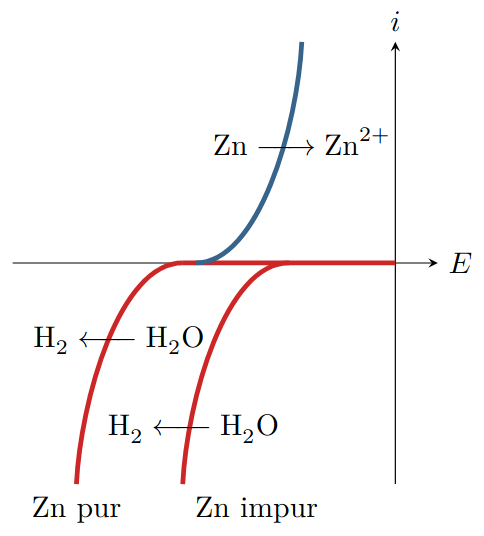
\includegraphics[width=0.55\linewidth]{corrosion_zinc.png}
	\caption{Courbes courant-potentiel associées à la corrosion du zinc pur et impur. Source : poly de cours de Etienne Thibierge.}
\end{figure}








\end{document}
